\section{Simul'ari}

\subsection*{LTSpice}

LTSpice este un simulator de circuite, 'in care circuitele pot fi descrise ca un fi'sier text cu o list'a de elemente, numit \textit{netlist} sau ca o schema de circuit (desen), numit'a \textit{schematics} \cite{ltspice}. Este util'a 'in'telegerea modului de lucru 'in ambele variante, avantajele 'si dezavantajele lor.

 \begin{itemize}
 \item[--] Lucrul cu \textit{netlist} are avantajul c'a fi'sierul generat este portabil ('in propor'tie destul de mare) 'intre diferitele simulatoare de circuite (PSpice, LTSpice, ngspice, etc.). Dac'a schema este foarte complicat'a, lucrul cu acest fi'sier devine greoi, eventualele gre'seli fiind greu de depistat. 'In plus, este necesar'a cunoa'sterea precis'a a sintaxei. 
 \begin{example}[Fi'sier netlist corespunz'ator circuitului din Fig. \ref{fig:comparator_cu_divizor}]
\textcolor{white}{!}\\
\textcolor{OliveGreen}{* circuit comparator cu tensiunea de referinta}\\
\textcolor{OliveGreen}{* data de un divizor de tensiune}\\
R1 b 0 10k \\
C1 b 0 470uf IC=12V \\
R3 V+ N001 1k \\
R4 N001 0 1k \\
XU1 N001 b V+ V- c LT1017 \\
R2 P001 c 1k \\
D1 P001 0 D \\
D2 0 P002 D \\
R5 V+ c 470 \\
R6 c P002 1k \\
R7 V+ a 10\\
V1 V+ 0 12V\\ 
V2 0 V- 12V \\
%\textcolor{blue}{.model D D /Library/Application Support/LTspice/lib/cmp/standard.dio }\\
\textcolor{blue}{.tran 10s uic} \\
%\textcolor{blue}{.lib LTC1.lib}\\
%\textcolor{blue}{.backanno}\\
\textcolor{blue}{.end}\\
\end{example} 

\item[--] Lucrul cu \textit{schematics} are avantajul c'a este intuitiv. Dezavantajul provine din faptul c'a fi'sierul generat nu este portabil 'intre diferite simulatoare. Dac'a se dore'ste 'ins'a migrarea c'atre un alt simulator, atunci se poate exporta netlistul asociat. Un alt dezavantaj este acela c'a, 'in cazul elementelor nepolarizate (de ex. rezistoarele), utilizatorul nu are un control imediat al sensului de referin't'a al laturii. Pentru a 'in'telege acest sens de referin't'a trebuie inspectat netlistul.
 \end{itemize} 
 
\subsection*{Hands-on it!}

Vom exemplifica generarea unui netlist pentru un divizor de tensiune rezistiv, 'in gol, format din dou'a rezistoare $R_1 = 360~\Omega$ 'si $R_2 = 180~\Omega$, la bornele c'aruia se aplic'a o tensiune de 6 V, ca in Fig. \ref{fig:spice_ex1_1_2} st\^anga. 

\begin{figure}
	\centering
		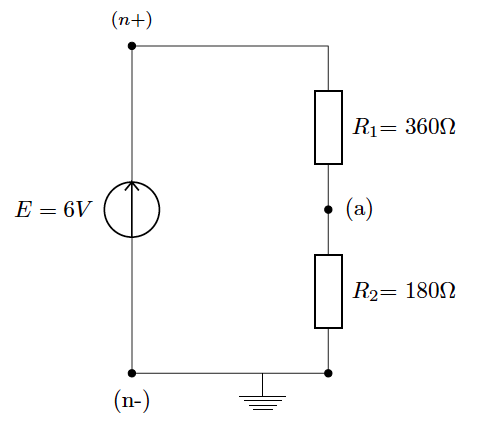
\includegraphics[width=0.5\textwidth]{laborator_01/figuri/spice_divizor_gol_ex1}
		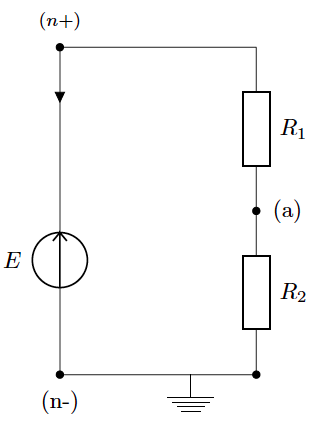
\includegraphics[width=0.33\textwidth]{laborator_01/figuri/spice_divizor_gol_ex1_crt}
	\caption{Divizor de tensiune 'in gol, exemplu. St\^anga: circuit cu noduri etichetate, dreapta: sens curent pentru SIT.}
	\label{fig:spice_ex1_1_2}
\end{figure}

Pentru crearea netlistului, circuitul trebuie preg'atit astfel:
\begin{enumerate}
\item Se pun noduri la bornele tuturor elementelor de circuit.
\item Se alege un nod la mas'a 'si se eticheteaz'a nodurile. Eticheta nodului de mas'a va fi obligatoriu 0.
\item Se aleg sensuri de referin't'a pentru curen'ti. Fiecare latur'a devine orientat'a, de la un nod ini'tial la un nod final.

\begin{retine}
  \label{retine3_1}
  \index{}
    'In cazul surselor ideale de tensiune este obligatorie reprezentarea sensului de referin't'a al curentului ca 'in Fig. \ref{fig:spice_ex1_1_2} dreapta.
\end{retine}

%\begin{figure}
%	\centering
%		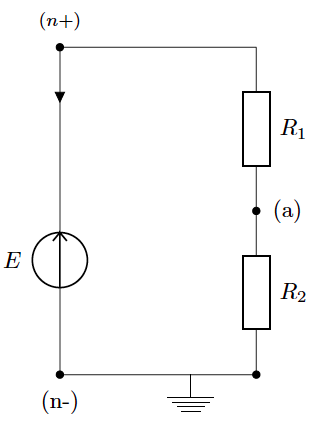
\includegraphics[width=0.3\textwidth]{laborator_01/figuri/spice_divizor_gol_ex1_crt}
%	\caption{Divizor de tensiune 'in gol -- sens curent pentru SIT.}
%	\label{fig:spice_ex1_2}
%\end{figure}

\item Se scrie fi'sierul netlist (numit de ex. divizorTensiuneGol.cir): \\
\textcolor{OliveGreen}{* Divizorul de tensiune} \\
\textcolor{OliveGreen}{* in gol}

\begin{figure}[!b]
	\centering
		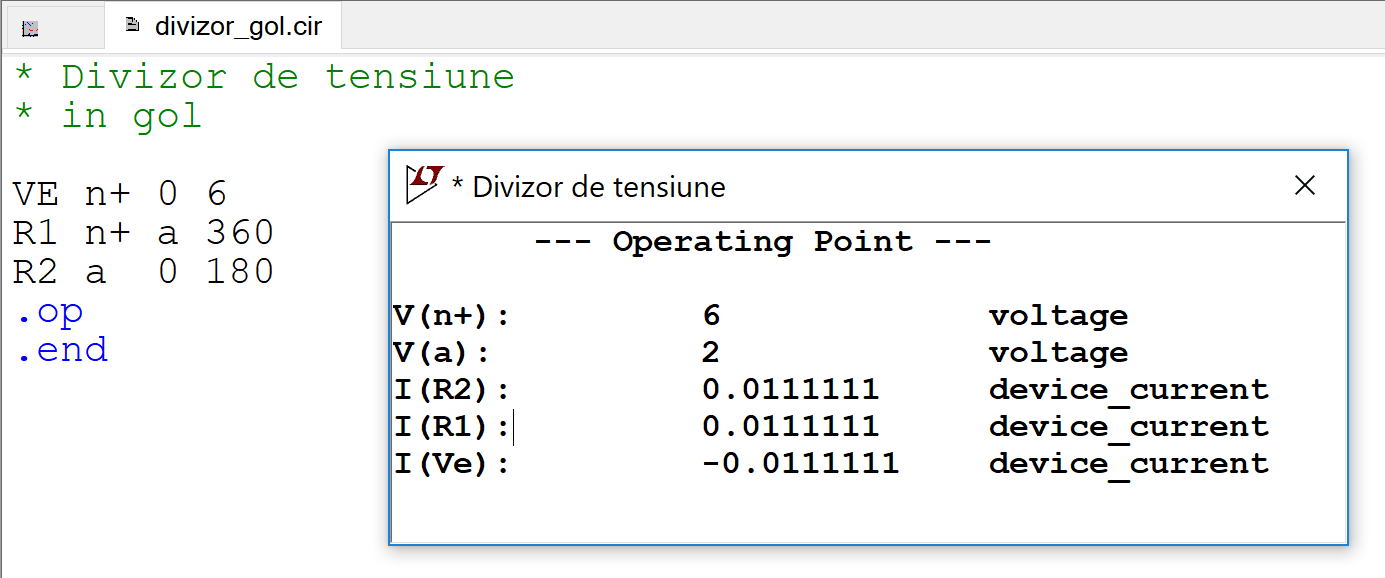
\includegraphics[width=0.7\textwidth]{laborator_01/figuri/spice_divizor_gol_op}
	\caption{Divizor de tensiune 'in gol -- rezultatul simul'arii.}
	\label{fig:spice_ex1_3}
\end{figure}
\begin{figure}[!b]
	\centering
		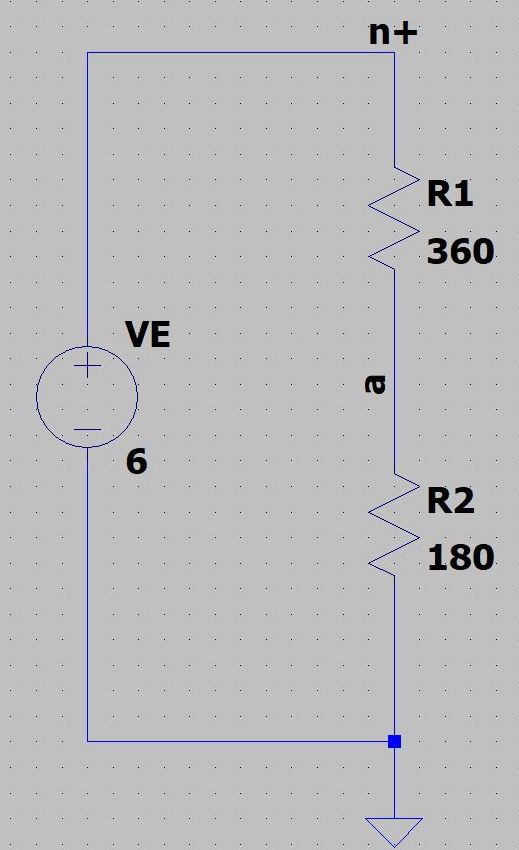
\includegraphics[width=0.33\textwidth]{laborator_01/figuri/spice_divizor_schematics}
	\caption{Divizor de tensiune 'in gol -- circuitul 'in \textit{schematics}.}
	\label{fig:spice_ex1_4}
\end{figure}

VE n+ 0 6 \\
R1 n+ a 360 \\
R2 a  0 180 \\
\textcolor{blue}{.op} \\
\textcolor{blue}{.end} 

\begin{itemize}
\item[--] Liniile care 'incep cu * reprezint'a comentarii.
\item[--] Prima linie din fi'sier este intotdeauna interpretat'a ca un comentariu.
\item[--] Fiecare linie reprezint'a o latura (un element).
\item[--] Primul caracter al unei linii indic'a tipul elementului (de ex. V pentru SIT, R pentru rezistor).
\item[--] Sintaxa liniei de tip SIT este:

$\mathrm{V_{nume}~~n+~~n-~~valoare}$

unde \textit{n+} reprezint'a nodul ini'tial al laturii, \textit{n-} reprezint'a nodul final, iar \textit{valoare} reprezint'a tensiunea electromotoare.
\item[--] Sintaxa liniei de tip R este:

$\mathrm{R_{nume}~~n+~~n-~~valoare}$

unde \textit{n+} reprezint'a nodul ini'tial al laturii, \textit{n-} reprezint'a nodul final, iar \textit{valoare} reprezint'a rezisten'ta. 
\item[--] Nodul de mas'a are intotdeauna eticheta 0 'si trebuie s'a existe 'in circuit.
\item[--] Liniile care 'incep cu . reprezint'a directive SPICE. 'In cazul exemplului studiat, \textit{.op} este o directiv'a de simulare 'in c.c. (o.p. = \textit{operational point} = \textit{punct static de func'tionare})
\item[--] Liniile de dup'a \textit{.end} sunt ignorate.

\end{itemize}
\end{enumerate}

Rezultatul simul'arii acestui netlist este Fig. \ref{fig:spice_ex1_3}. Observa'ti c'a $V_a = 2~\mathrm{V}$, a'sa cum era as'teptat, divizorul fiind cu 3.

\begin{figure}
	\centering
		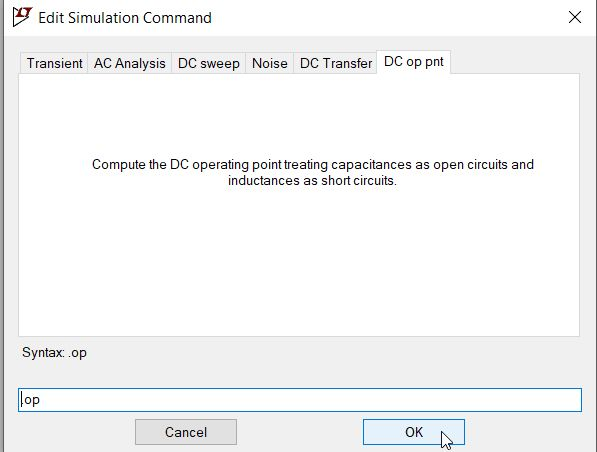
\includegraphics[width=0.45\textwidth]{laborator_01/figuri/spice_divizor_comanda_simulare}
	\caption{Divizor de tensiune 'in gol -- fereastr'a de stabilire a tipului de simulare.}
	\label{fig:spice_ex1_5}
\end{figure}

Generarea schemei se face intuitiv, printr-o interfa't'a grafic'a (Fig. \ref{fig:spice_ex1_4}). Rularea se face apasand pe butonul Run 
\includegraphics[width=0.03\textwidth]{laborator_01/figuri/spice_Run_icon}. Dac'a a fost omis'a comanda de simulare, atunci programul conduce automat c'atre o fereastr'a de unde se stabile'ste tipul de simulare (Fig. \ref{fig:spice_ex1_5}).

'In schematics, etichetarea unui nod se face din Meniul \textbf{Edit $\rightarrow$ Label Net} sau direct cu \textbf{F4}, iar generarea fi'sierului netlist se face din meniul \textbf{View $\rightarrow$ SPICE Netlist}. Netlist-ul poate fi salvat ca fi'sier separat pentru modific'ari ulterioare cu click-dreapta 'in fereastr'a 'si alegerea \textbf{Edit as Independent netlist}.

Mai multe detalii despre SPICE se g'asesc 'in \cite{ltspice} 'si \cite{ltspicewiki}.

\begin{definition}[facultativ] Toleran'te 'in Spice\\
LTSpice permite descrierea elementelor cu toleran'te, una dintre metode fiind analiza Monte Carlo (Fig. \ref{fig:spice_tolerante}). Se definesc trei parametri care reprezint'a toleran'tele pentru $R_1$, $R_2$ 'si $U$. Valorile celor trei m'arimi sunt 'inlocuite cu un model Monte Carlo, care pentru sintaxa $mc(val,tol)$ variaz'a valoarea $val$ aleatoriu conform unei distribu'tii uniforme 'intre $val(1+tol)$ 'si $val(1-tol)$. 'In concluzie, aceste valori reprezint'a marginile erorilor relative ale elementelor (toleran'tele).\\

Vom considera c'a rezistoarele au toleran'ta 5\%, iar tensiunea de alimentare $U$ are marginea erorii absolute egal'a cu $0.1$ V. Remarca'ti c'a de aceast'a dat'a este dat'a eroarea absolut'a pentru tensiunea de intrare, nu cea relativ'a ca p\^an'a acum. Toleran'tele definite in Spice sunt relative, deci trebuie calculat'a marginea erorii relative pentru $U$, care este:
\begin{equation*} 
r_U = \frac{a_U}{U} = 0.0167 = 1.67\%.
\end{equation*}

Directiva:\\
.step param run 1 500 1 \\
arat'a c'a se vor executa 500 de simul'ari, fiecare simulare folosind pentru valori diferite ale elementelor. 

Forma general'a a acestei directive SPICE este: \\
.step param \textless nume parametru\textgreater \textless start\textgreater \textless stop\textgreater \textless pas\textgreater\\

Dac'a din Fig. \ref{fig:spice_tolerante} alegem valoarea minim'a 'si valoarea maxim'a pentru tensiunea de ie'sire $U_2 = V_a$, putem calcula marginea erorii relative care nu ar trebui s'a dep'a'seasc'a valoarea calculat'a de 11.7\%.
Pentru exemplul considerat, valoarea $U_2 = V_a \in [1.861, 2.1326], V_a \in \left[2-6.91\%, 2+6.63\%\right]$.\\

Putem analiza 'in Spice 'si cazul cel mai defavorabil (\textit{worst-case scenario}), 'in care datele au valorile minime 'si maxime. Pentru acest lucru 'inlocuim modelul Monte Carlo cu o func'tie proprie, care pentru prima execu'tie 'intoarce valorile nominale, iar pentru urm'atoarele execu'tii 'intoarce aleatoriu valorile minime sau maxime pentru cele trei m'arimi (func'tia \textit{flat} 'intoarce un num'ar aleatoriu 'intre -1 'si 1).\\

Fig. \ref{fig:spice_tolerante_wc} con'tine schema 'si rezultatele pentru 50 de simulari de acest tip. Valorile tensiunii de ie'sire sunt 'in intervalul $[1.8365, 2.17]$, ceea ce corespunde unei erori relative de $V_a \in \left[2-6.95\%, 2+7.325\%\right]$.
\end{definition} 

\begin{figure}[t]
	\centering
		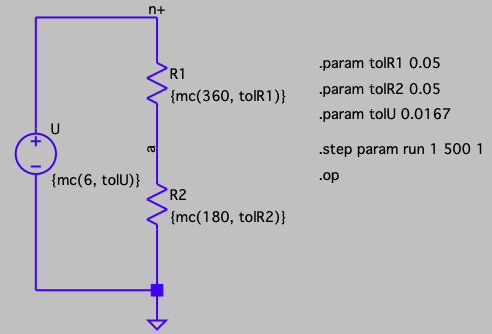
\includegraphics[width=0.42\textwidth]{laborator_01/figuri/spice_schematics_tolerante}
		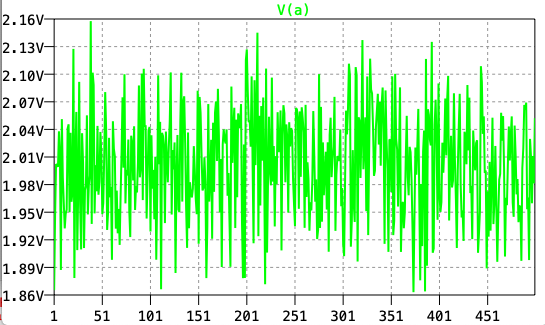
\includegraphics[width=0.5\textwidth]{laborator_01/figuri/spice_rezultate_tolerante}
	\caption{Divizor de tensiune 'in gol -- m'arimi cu toleran'te, schematics 'si rezultate.}
	\label{fig:spice_tolerante}
\end{figure}
\begin{figure}[t]
	\centering
		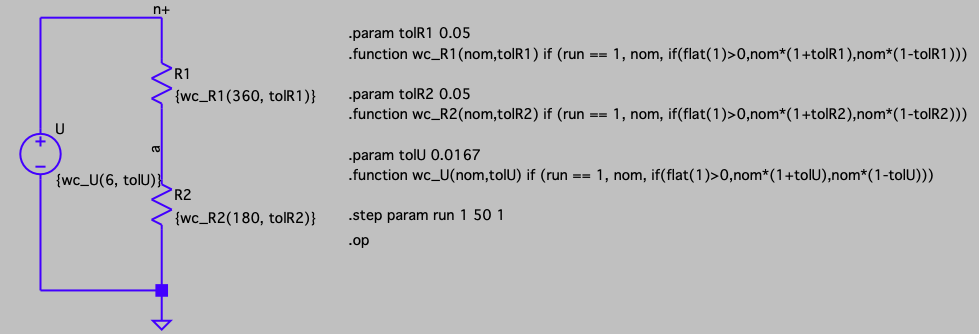
\includegraphics[width=0.7\textwidth]{laborator_01/figuri/spice_schematics_tolerante_wc}\\
		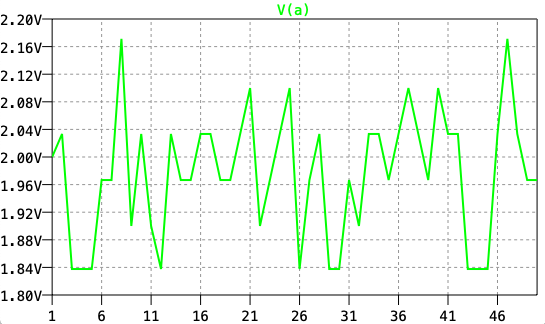
\includegraphics[width=0.7\textwidth]{laborator_01/figuri/spice_rezultate_tolerante_wc}
	\caption{Divizor de tensiune 'in gol -- m'arimi cu toleran'te, ''worst-case scenario'', schematics 'si rezultate.}
	\label{fig:spice_tolerante_wc}
\end{figure}
\begin{figure}[b]
	\centering
		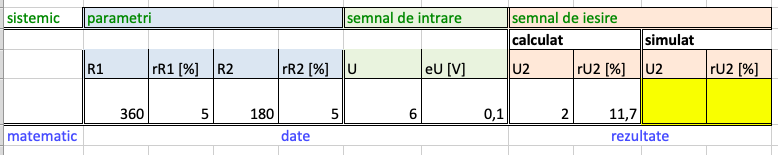
\includegraphics[width=\textwidth]{laborator_01/figuri/divizor_tensiune_excel2}
	\caption{Divizor de tensiune 'in gol -- foaie de calcul cu m'arimi calculate 'si simulate.}
	\label{fig:divizor_tensiune_excel2}
\end{figure}

'In acest moment putem preg'ati o foaie de calcul 'in care s'a trecem valorile calculate 'si valorile rezultate 'in urma simul'arii, ca in Fig. \ref{fig:divizor_tensiune_excel2}.


\begin{exercise}[fi'sier \textit{.cir} sau \textit{.asc}, fi'sier \textit{.xls}, 'inainte de laborator]
  Analiza'ti 'si simula'ti divizorul de tensiune 'in sarcin'a. Preg'ati'ti o foaie de calcul potrivit'a.
\end{exercise}
\begin{exercise}[fi'sier \textit{.cir} sau \textit{.asc}, fi'sier \textit{.xls}, 'inainte de laborator]
  Analiza'ti 'si simula'ti puntea rezistiv'a. Preg'ati'ti o foaie de calcul potrivit'a.
\end{exercise}

